\documentclass[b5paper,papersize,11pt,dvipdfmx]{jsarticle}
\usepackage[dvipdfmx]{graphicx}
\usepackage{tikz}

\begin{document}

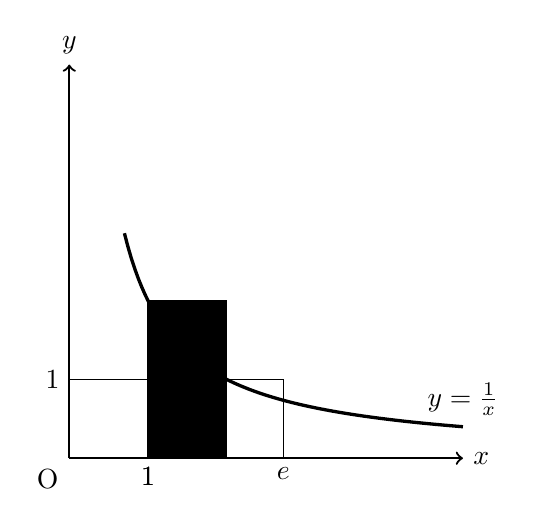
\begin{tikzpicture}[domain=0:5, samples=100, very thick] % 定義域、点の数、線幅
  \draw (0,0) node[below left]{O}; % 原点、0でも、above, below, left, rightで位置指定
  % 位置指定はanchor=north, south, east, westでも可能
  \draw[thick, ->] (0,0)--(5,0) node[right] {$x$}; % x軸、[->]で矢印、他に[-stealth]等
  \draw[thick, ->] (0,0)--(0,5) node[above] {$y$}; % y軸
  \draw [domain=0.7:5] plot(\x, 2/\x) node[above] {$y=\frac1x$};
  \draw [thin](0,1) node [left]{$1$}--(e,1)--(e,0) node[below]{$e$}; % 補助線
  \draw [thin](1,0) node [below]{$1$}--(1,1);
  \draw [thin](1,0) node [below]{$1$}--(1,2)--(2,2)--(2,0);
  \fill (1,0)--(1,2)--(2,2)--(2,0);
\end{tikzpicture}


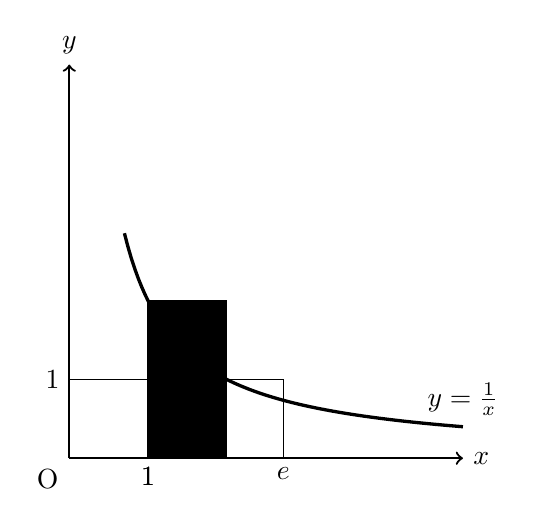
\begin{tikzpicture}[domain=0:5, samples=100, very thick] % 定義域、点の数、線幅
  \draw (0,0) node[below left]{O}; % 原点、0でも、above, below, left, rightで位置指定
  % 位置指定はanchor=north, south, east, westでも可能
  \draw[thick, ->] (0,0)--(5,0) node[right] {$x$}; % x軸、[->]で矢印、他に[-stealth]等
  \draw[thick, ->] (0,0)--(0,5) node[above] {$y$}; % y軸
  \draw [domain=0.7:5] plot(\x, 2/\x) node[above] {$y=\frac1x$};
  \draw [thin](0,1) node [left]{$1$}--(e,1)--(e,0) node[below]{$e$}; % 補助線
  \draw [thin](1,0) node [below]{$1$}--(1,1);
  \draw [thin](1,0) node [below]{$1$}--(1,2)--(2,2)--(2,0);
  \fill (1,0)--(1,2)--(2,2)--(2,0);
\end{tikzpicture}


\end{document}